\everymath{\displaystyle}

%%%%%%%%%%%%%%%%%%%%%%%%%%%%%%%%%%%%%%%%
%           main body
%%%%%%%%%%%%%%%%%%%%%%%%%%%%%%%%%%%%%%%%

%-----------------------------------
%	TITLE PAGE
%-----------------------------------

\title[第八章\\
反常积分]{\texorpdfstring{\LARGE \bfseries 第八章\quad 反常积分}{第八章 反常积分}} % The short title appears at the bottom of every slide, the full title is only on the title page
\author[\smaller \S 8.2\\
收敛判别法] % Your institution as it will appear on the bottom of every slide, maybe shorthand to save space
{\Large \bfseries \S 8.2 反常积分的收敛判别法}
% \author{Singular Value Decomposition} % Your name
% \date{\today} % Date, can be changed to a custom date
\date{}

%------------------------------------------------

\begin{document}

%------------------------------------------------

\begin{frame}

\titlepage % Print the title page as the first slide

\end{frame}

%------------------------------------------------

% \begin{frame}
% \frametitle{内容提要} % Table of contents slide, comment this block out to remove it
% \tableofcontents % Throughout your presentation, if you choose to use \section{} and \subsection{} commands, these will automatically be printed on this slide as an overview of your presentation
% \end{frame}

%-----------------------------------
%	PRESENTATION SLIDES
%-----------------------------------

%------------------------------------------------

\begin{frame}{绪言}

{
\larger[1]

考虑反常积分
\begin{equation*}
\int_a^{\omega} f(x) ~ \mathrm{d} x, \quad \text{$\omega$ 是无穷或者 $f(x)$ 的奇点.}
\end{equation*}
有时候, 我们不需要 (往往也不容易) 计算某个反常积分的值, 但需要 (\alert{定性地}) 判断它是否收敛, 所以我们发展处一系列判别法, 来判断一个反常积分的敛散性.
}

\end{frame}

%------------------------------------------------

\section{反常积分的 Cauchy 收敛原理}

%------------------------------------------------

\begin{frame}
\frametitle{Cauchy 收敛原理}

由于反常积分定义是用极限表达的, 最基本的判别准则为

\begin{thm}[Cauchy 收敛原理]
反常积分 $\displaystyle \int_a^{\omega} f(x) ~ \mathrm{d} x$ 收敛 ($\omega$ 是无穷或者 $f(x)$ 的奇点) 的充要条件是: $\forall~\varepsilon > 0,$
\begin{itemize}
\item $\omega$ 是无穷: $\exists ~ X > a,$ 使得 $\forall~c_2 > c_1 > X,$
\item $\omega$ 是奇点: $\exists ~ \delta > 0,$ 使得 $\forall~\omega > c_2 > c_1 > \omega - \delta,$
\end{itemize}
有 $\displaystyle \left| \int_{c_1}^{c_2} f(x) ~ \mathrm{d}x \right| < \varepsilon.$
\end{thm}

\pause

% \alert{关键在于}, $\displaystyle \left| \int_{c_1}^{c_2} f(x) ~ \mathrm{d}x \right|$ 的估计.

\begin{eg}
讨论 $\displaystyle \int_a^{+\infty} \dfrac{1}{\nroot[n]{x^4 + 3x^3 + 5x^2 + 2x - 1}} ~ \mathrm{d} x$ 的敛散性
\end{eg}

\alert{提示:} 对充分大的 $x,$ 对分母进行放缩, 进而控制 $\displaystyle \left| \int_{c_1}^{c_2} f(x) ~ \mathrm{d}x \right|.$

\end{frame}

%------------------------------------------------

\begin{frame}

\begin{question}
之前判断函数是否 Riemann 可积时, 利用振幅判别法, 有
\begin{equation*}
f(x) \in \mathfrak{R}[a, b] \quad \stackanchor[6pt]{$\implies$}{$\bcancel{\Longleftarrow}$} \quad |f(x)| \in \mathfrak{R}[a, b]
\end{equation*}
那么反常积分的情况如何?
\end{question}

\pause

一方面, 有 $\displaystyle \left| \int_{c_1}^{c_2} f(x) ~ \mathrm{d}x \right| \leqslant \int_{c_1}^{c_2} |f(x)| ~ \mathrm{d}x,$ 那么由 \alert{Cauchy 收敛原理}知
\begin{empheq}[box={\fancymath[colback=cyan!30, drop lifted shadow, sharp corners]}]{equation*}
\text{$f(x)$ 反常积分收敛 $\Longleftarrow$ $|f(x)|$ 反常积分收敛}
\end{empheq}

\pause

另一方面, 考虑函数定义在 $[1, +\infty)$ 上的函数 $f(x) = (-1)^{[x]+1} \frac{1}{[x]},$ 可知
\begin{empheq}[box={\fancymath[colback=cyan!30, drop lifted shadow, sharp corners]}]{equation*}
\text{$f(x)$ 反常积分收敛 $\bcancel{\implies}$ $|f(x)|$ 反常积分收敛}
\end{empheq}

\end{frame}

%------------------------------------------------

\begin{frame}

\frametitle{绝对可积与条件可积函数}

\begin{block}{绝对可积（绝对收敛）}
设函数 $f(x)$ 在 $[a, \omega)$ 上\emph{局部可积} (即在每个闭区间 $[a, b] \subset [a, \omega)$ 上 Riemann 可积), 若反常积分
\begin{equation*}
\int_a^{+\infty} |f(x)| ~ \mathrm{d}x \ \text{收敛}
\end{equation*}
则称 $f(x)$ 在 $[a, \omega)$ 上\alert{绝对可积}, 称反常积分 $\int_a^{\omega}f(x) ~ \mathrm{d} x$ \alert{绝对收敛}.
\end{block}

\begin{block}{条件可积（条件收敛）}
若 $\int_a^{\omega}f(x) ~ \mathrm{d} x$ 收敛, 但$\int_a^{\omega}|f(x)| ~ \mathrm{d} x$ 发散, 则称 $f(x)$ \alert{条件可积}, 称反常积分 $\int_a^{\omega}f(x) ~ \mathrm{d} x$ \alert{条件收敛}.
\end{block}

\pause

\alert{注意:} 条件收敛与绝对收敛下, 反常积分 $\displaystyle \int_a^{\omega}f(x) ~ \mathrm{d} x$ 都是收敛的.

\end{frame}

%------------------------------------------------

\section{非负函数反常积分的收敛判别法}

%------------------------------------------------

\begin{frame}
\frametitle{比较判别法}

先来看最简单的情况, 即被积函数 $f(x)$ 是非负函数.

\pause

\begin{thm}[比较判别法]
设函数 $f(x), \varphi(x)$ 在 $[a, \omega)$ 上局部可积, 并且在 $[a, \omega)$ 上恒有 $0 \leqslant f(x) \leqslant \varphi(x),$ 那么
\begin{itemize}
\item $\int_a^{\omega} \varphi(x) ~ \mathrm{d} x$ 收敛 $\implies$ $\int_a^{\omega} f(x) ~ \mathrm{d} x$ 收敛;
\item $\int_a^{\omega} f(x) ~ \mathrm{d} x$ 发散 $\implies$ $\int_a^{\omega} \varphi(x) ~ \mathrm{d} x$ 发散.
\end{itemize}
且有 $\displaystyle \int_a^{\omega} f(x) ~ \mathrm{d} x \leqslant \int_a^{\omega} \varphi(x) ~ \mathrm{d} x.$ (也包含了发散的情况, 即积分无穷大的情况.)
\end{thm}

\pause

\begin{remark}
比较判别法的核心在于, 通过比较一个反常积分的被积函数与另一个反常积分的被积函数的大小关系, 来判断前者的敛散性. 这就要求我们能够找到一个合适的比较函数 $\varphi(x)$, 使得 $f(x) \leqslant \varphi(x)$ 并且 $\int_a^{\omega} \varphi(x) ~ \mathrm{d} x$ 的敛散性是已知的.
\end{remark}

\end{frame}

%------------------------------------------------

\begin{frame}
\frametitle{比较判别法的本质}

比较判别法的证明, 主要考察的是变上限积分函数
\[
F(x) := \int_a^x f(t) ~ \mathrm{d} t, \quad \Phi(x) := \int_a^x \varphi(t) ~ \mathrm{d} t.
\]
它们是定义在 $[a, \omega)$ 上的单调非减函数.

$f(x)$ 的可积性可以归纳为极限 $\displaystyle \lim_{x \to \omega} F(x)$ 的存在性, 又可以进一步归纳为 $F(x)$ 的有界性:

\begin{prop}
设 $f(x)$ 在 $[a, \omega)$ 上非负, 且局部可积, $F(x) := \int_a^x f(t) ~ \mathrm{d} t,$ 那么
\[
\text{反常积分} ~ \int_a^{\omega} f(x) ~ \mathrm{d} x ~ \text{收敛} \quad \Longleftrightarrow \quad F(x) ~ \text{有界.}
\]
\end{prop}

\end{frame}

%------------------------------------------------

\begin{frame}
\frametitle{比较判别法的推论}

\begin{cor}
设 $f(x)$ 在 $[1, +\infty)$ 上非负不增, 且局部可积, 那么级数 $\displaystyle \sum_{n=1}^{\infty} f(n)$ 与反常积分 $\displaystyle \int_1^{+\infty} f(x) ~ \mathrm{d} x$ 同敛散.
\end{cor}

\pause

\startproof[bg=yellow, fg=red]
由于 $f(x)$ 在 $[1, +\infty)$ 上非负不增, 则对于任意的 $n \in \mathbb{N}^+$ 和 $x \in [n, n+1),$ 有
\[
f(n+1) \leqslant f(x) \leqslant f(n).
\]
因此
\[
f(n+1) = \int_n^{n+1} f(n+1) ~ \mathrm{d} x \leqslant \int_n^{n+1} f(x) ~ \mathrm{d} x \leqslant \int_n^{n+1} f(n) ~ \mathrm{d} x = f(n).
\]
两端求和得
\[
\sum_{n=1}^{N} f(n+1) \leqslant \int_1^{N+1} f(x) ~ \mathrm{d} x \leqslant \sum_{n=1}^{N} f(n).
\]
这就说明了 $\displaystyle \sum_{n=1}^{\infty} f(n)$ 与 $\displaystyle \int_1^{+\infty} f(x) ~ \mathrm{d} x$ 同敛散.
\qed

\end{frame}

%------------------------------------------------

\begin{frame}
\frametitle{比较判别法的推论}

\begin{cor}
取 $f(x) = \frac{1}{x^s}$, 则 $\displaystyle \zeta(s) := \sum_{n=1}^{\infty} \frac{1}{n^s}$ 与 $\displaystyle \int_1^{+\infty} \frac{1}{x^s} ~ \mathrm{d} x$ 同敛散. 因此 $\zeta(s)$ 在 $s > 1$ 时收敛, 在 $s \leqslant 1$ 时发散.
\end{cor}

\pause
\vspace{0.5em}

若取 $s = a + bi$ 为复数, 则
\[
\sum_{n=1}^{\infty} \frac{1}{n^s} ~ \text{绝对收敛} \quad \Longleftrightarrow \quad \Re(s) > 1.
\]

\end{frame}

%------------------------------------------------

\begin{frame}
\frametitle{比较判别法的极限形式}

\begin{cor}[比较判别法的极限形式]
设 $f(x), \varphi(x)$ 在 $[a, \omega)$ 上非负且局部可积, 且 $\displaystyle \lim_{x \to \omega} \frac{f(x)}{\varphi(x)} = \ell,$ 那么
\begin{itemize}
\item 若 $0 \leqslant \ell < +\infty,$ 则 $\int_a^{\omega} \varphi(x) ~ \mathrm{d} x$ 收敛 $\implies$ $\int_a^{\omega} f(x) ~ \mathrm{d} x$ 收敛;
\item 若 $0 < \ell \leqslant +\infty,$ 则 $\int_a^{\omega} f(x) ~ \mathrm{d} x$ 收敛 $\implies$ $\int_a^{\omega} \varphi(x) ~ \mathrm{d} x$ 收敛.
\end{itemize}
特别地, 当 $\ell \in (0, +\infty)$ 时, $\int_a^{\omega} f(x) ~ \mathrm{d} x$ 与 $\int_a^{\omega} \varphi(x) ~ \mathrm{d} x$ 同敛散.
\end{cor}

\pause

\startproof[bg=yellow, fg=red]
对 $\omega = +\infty$ 的情况进行证明.

(1) 若 $\ell < +\infty,$ 则存在 $M > 0,$ 使得 $\forall~x > M,$ 有 $\frac{f(x)}{\varphi(x)} < \ell + 1.$ 因此 $\forall~x > M,$ 有 $f(x) < (\ell + 1) \varphi(x).$ 由比较判别法知 $\int_a^{\omega} \varphi(x) ~ \mathrm{d} x$ 收敛 $\implies$ $\int_a^{\omega} f(x) ~ \mathrm{d} x$ 收敛.

\end{frame}

%------------------------------------------------

\begin{frame}
\frametitle{比较判别法的极限形式}

(2) 若 $\ell > 0,$ 则存在 $M > 0,$ 使得 $\forall~x > M,$ 有 $\frac{f(x)}{\varphi(x)} > \frac{\ell}{2}.$ 因此 $\forall~x > M,$ 有 $f(x) > \frac{\ell}{2} \varphi(x).$ 由比较判别法知 $\int_a^{\omega} f(x) ~ \mathrm{d} x$ 收敛 $\implies$ $\int_a^{\omega} \varphi(x) ~ \mathrm{d} x$ 收敛.
\qed

\pause
\vspace{1em}

\begin{eg}
讨论 $\displaystyle \int_1^{+\infty} \frac{1}{\sqrt[3]{x^4 + 3x^3 + 5x^2 + 2x - 1}} ~ \mathrm{d} x$ 的敛散性.
\end{eg}

\pause
\vspace{0.5em}

\startproof[bg=yellow, fg=red](解)
对于充分大的 $x,$ 分母满足 $\sqrt[3]{x^4 + 3x^3 + 5x^2 + 2x - 1} \sim \sqrt[3]{x^4} = x^{\frac{4}{3}}.$ 因此, 由比较判别法的极限形式知, $\displaystyle \int_1^{+\infty} \frac{1}{\sqrt[3]{x^4 + 3x^3 + 5x^2 + 2x - 1}} ~ \mathrm{d} x$ 与 $\displaystyle \int_1^{+\infty} \frac{1}{x^{\frac{4}{3}}} ~ \mathrm{d} x$ 同敛散. 后者收敛, 因此前者也收敛.
\qed

\end{frame}

%------------------------------------------------

\begin{frame}
\frametitle{比较判别法应用举例}

\begin{eg}
讨论 $\displaystyle \int_1^{+\infty} e^{-x^2/2} ~ \mathrm{d} x$ 的敛散性.
\end{eg}

\pause
\vspace{0.5em}

\startproof[bg=yellow, fg=red](解)
在 $[1, +\infty)$ 上, 有 $0 < e^{-x^2/2} < e^{-x/2}$ 恒成立. 而
\[
\int_1^{+\infty} e^{-x/2} ~ \mathrm{d} x = 2e^{-1/2} < +\infty,
\]
因此, 由比较判别法知 $\displaystyle \int_1^{+\infty} e^{-x^2/2} ~ \mathrm{d} x$ 收敛.
\qed

\pause
\vspace{0.5em}

由 $\displaystyle \int_1^{+\infty} e^{-x^2/2} ~ \mathrm{d} x$ 收敛易知 $\displaystyle \int_{-\infty}^{+\infty} e^{-x^2/2} ~ \mathrm{d} x$ 也是收敛的. 事实上, $\displaystyle I := \int_{-\infty}^{+\infty} e^{-x^2/2} ~ \mathrm{d} x$ 的值很容易计算 (要利用一些重积分的技巧):
\begin{align*}
I^2 & = \int_{-\infty}^{+\infty} e^{-x^2/2} ~ \mathrm{d} x \int_{-\infty}^{+\infty} e^{-y^2/2} ~ \mathrm{d} y = \int_{-\infty}^{+\infty} \int_{-\infty}^{+\infty} e^{-(x^2 + y^2)/2} ~ \mathrm{d} x \mathrm{d} y \\
& = \int_0^{2\pi} \int_0^{+\infty} e^{-r^2/2} r ~ \mathrm{d} r \mathrm{d} \theta = 2\pi.
\end{align*}

\end{frame}

%------------------------------------------------

\begin{frame}
\frametitle{比较判别法应用举例}

记 $\varphi(x) := \frac{1}{\sqrt{2\pi}} e^{-x^2/2}$, 则 $\displaystyle \int_{-\infty}^{+\infty} \varphi(x) ~ \mathrm{d} x = 1.$ $\varphi(x)$ 正是\emph{标准正态分布}的概率密度函数.

\pause
\vspace{0.5em}

\begin{eg}
椭圆积分 $\displaystyle \int_0^1 \frac{1}{\sqrt{(1-x^2)(1-k^2 x^2)}} ~ \mathrm{d} x$ 是收敛的. 原因是, 当 $x \to 1^-$ 时, 被积函数的分母
\[
\sqrt{(1-x^2)(1-k^2 x^2)} \sim \sqrt{2(1-k^2)} (1 - x)^{\frac{1}{2}}.
\]
因此, 由比较判别法的极限形式知, $\displaystyle \int_0^1 \frac{1}{\sqrt{(1-x^2)(1-k^2 x^2)}} ~ \mathrm{d} x$ 与 $\displaystyle \int_0^1 \frac{1}{\sqrt{1 - x}} ~ \mathrm{d} x$ 同敛散. 后者收敛, 因此前者也收敛.
\end{eg}

\end{frame}

%------------------------------------------------

\begin{frame}
\frametitle{Cauchy 判别法}

将刚才例子中讨论的反常积分敛散性的过程进行总结, 就得到了 Cauchy 判别法:

\begin{thm}[Cauchy 判别法]
设 $f(x)$ 在 $[a, +\infty) \subset [0, +\infty)$ 上非负且局部可积, $K > 0$ 为常数, 那么
\begin{itemize}
\item 若 $\displaystyle f(x) \leqslant \frac{K}{x^p}$, $p > 1,$ 则 $\displaystyle \int_a^{+\infty} f(x) ~ \mathrm{d} x$ 收敛;
\item 若 $\displaystyle f(x) \geqslant \frac{K}{x^p}$, $p \leqslant 1,$ 则 $\displaystyle \int_a^{+\infty} f(x) ~ \mathrm{d} x$ 发散.
\end{itemize}
\end{thm}

\pause
\vspace{0.5em}

\begin{cor}[Cauchy 判别法的极限形式]
设 $f(x)$ 在 $[a, +\infty) \subset [0, +\infty)$ 上非负且局部可积, $\displaystyle \lim_{x \to +\infty} x^p f(x) = \ell,$ 那么
\begin{itemize}
\item 若 $0 \leqslant \ell < +\infty,$ 且 $p > 1,$ 则 $\displaystyle \int_a^{+\infty} f(x) ~ \mathrm{d} x$ 收敛;
\item 若 $0 < \ell \leqslant +\infty,$ 且 $p \leqslant 1,$ 则 $\displaystyle \int_a^{+\infty} f(x) ~ \mathrm{d} x$ 发散.
\end{itemize}
\end{cor}

\end{frame}

%------------------------------------------------

\section{一般函数反常积分的收敛判别法}

%------------------------------------------------

\begin{frame}
\frametitle{Abel 判别法与 Dirichlet 判别法}

\begin{thm}
若以下两个条件之一满足, 则 $\displaystyle \int_a^{+\infty} f(x)g(x) ~ \mathrm{d} x$ 收敛:
\begin{itemize}
\item (Abel 判别法)
\begin{itemize}
\item (强条件) ~~ $\displaystyle \int_a^{+\infty} f(x) ~ \mathrm{d} x$ 收敛;
\item (弱条件) ~~ $g(x)$ 在 $[a, +\infty)$ 上单调有界.
\end{itemize}
\pause
\vspace{0.5em}
\item (Dirichlet 判别法)
\begin{itemize}
\item (弱条件) ~~ $F(x) := \int_a^x f(t) ~ \mathrm{d} t$ 在 $[a, +\infty)$ 上有界;
\item (强条件) ~~ $g(x)$ 在 $[a, +\infty)$ 上单调趋于零.
\end{itemize}
\end{itemize}
\end{thm}

\pause

看到被积函数的形式是 $f(x)g(x)$, 以及 $g(x)$ 满足的条件, 就想到要利用积分第二中值定理进行证明:
\[
f(x) ~ \text{可积}, g(x) ~ \text{单调} ~ \implies \int_a^b f(x)g(x) ~ \mathrm{d} x = g(a) \int_a^{\xi} f(x) ~ \mathrm{d} x + g(b) \int_{\xi}^b f(x) ~ \mathrm{d} x, \quad \text{其中}~\xi \in [a, b].
\]

\end{frame}

%------------------------------------------------

\begin{frame}
\frametitle{Abel 判别法证明}

积分第二中值定理: $\int_a^b f(x)g(x) ~ \mathrm{d} x = g(a) \int_a^{\xi} f(x) ~ \mathrm{d} x + g(b) \int_{\xi}^b f(x) ~ \mathrm{d} x$.

\vspace{1em}

若 $g(x)$ 进一步是有界的, 设 $G$ 为 $g(x)$ 的一个上界. 由于 $\displaystyle \int_a^{+\infty} f(x) ~ \mathrm{d} x$ 收敛, 则 $\forall ~ \varepsilon > 0,$ $\exists ~ A_0 > a,$ 使得 $\forall ~ A_2 > A_1 > A_0,$ 有
\[
\left| \int_{A_1}^{A_2} f(x) ~ \mathrm{d} x \right| < \frac{\varepsilon}{2G}.
\]
由积分第二中值定理知, $\exists ~ \xi \in [A_1, A_2],$ 使得
\[
\left| \int_{A_1}^{A_2} f(x)g(x) ~ \mathrm{d} x \right| = \left| g(A_1) \int_{A_1}^{\xi} f(x) ~ \mathrm{d} x + g(A_2) \int_{\xi}^{A_2} f(x) ~ \mathrm{d} x \right| < G \cdot \frac{\varepsilon}{2G} + G \cdot \frac{\varepsilon}{2G} = \varepsilon.
\]
由 Cauchy 收敛原理知 $\displaystyle \int_a^{+\infty} f(x)g(x) ~ \mathrm{d} x$ 收敛.
\qed

\end{frame}

%------------------------------------------------

\begin{frame}
\frametitle{Dirichlet 判别法证明}

积分第二中值定理: $\int_a^b f(x)g(x) ~ \mathrm{d} x = g(a) \int_a^{\xi} f(x) ~ \mathrm{d} x + g(b) \int_{\xi}^b f(x) ~ \mathrm{d} x$.

\vspace{1em}

设 $M$ 是 $F(x) := \int_a^x f(t) ~ \mathrm{d} t$ 的一个上界. 还是由积分第二中值定理知, $\forall ~ A_2 > A_1 \geqslant a$, $\exists ~ \xi \in [A_1, A_2],$ 使得
\[
\left| \int_{A_1}^{A_2} f(x)g(x) ~ \mathrm{d} x \right| = \left| g(A_1) \int_{A_1}^{\xi} f(x) ~ \mathrm{d} x + g(A_2) \int_{\xi}^{A_2} f(x) ~ \mathrm{d} x \right| < 2M |g(A_1)| + 2M |g(A_2)|.
\]
由于 $g(x)$ 在 $[a, +\infty)$ 上单调趋于零, 则 $\forall ~ \varepsilon > 0,$ $\exists ~ A_0 > a,$ 使得 $\forall ~ x > A_0$, 有 $|g(x)| < \frac{\varepsilon}{4M}.$ 取 $A_2 > A_1 > A_0,$ 则
\[
\left| \int_{A_1}^{A_2} f(x)g(x) ~ \mathrm{d} x \right| < 2M \cdot \frac{\varepsilon}{4M} + 2M \cdot \frac{\varepsilon}{4M} = \varepsilon.
\]
由 Cauchy 收敛原理知 $\displaystyle \int_a^{+\infty} f(x)g(x) ~ \mathrm{d} x$ 收敛.
\qed

\end{frame}

%------------------------------------------------

\begin{frame}
\frametitle{典型反常积分的敛散性判别}

\begin{eg}
讨论 $\displaystyle \int_1^{+\infty} \frac{\sin x}{x} ~ \mathrm{d} x$ 的敛散性.
\end{eg}

\pause

\startproof[bg=yellow, fg=red](解)
由 $\sin x$ 的周期性, 以及 $\displaystyle \int_{a}^{a+2\pi} \sin x ~ \mathrm{d} x = 0$ 可知, $\forall A > 1,$ $\displaystyle \left| \int_1^A \sin x ~ \mathrm{d} x \right|$ 有界. (或者直接由 $\displaystyle \int_1^A \sin x ~ \mathrm{d} x = \cos 1 - \cos A$ 可知) 又由于 $\displaystyle \lim_{x \to +\infty} \frac{1}{x} = 0,$ 则由 Dirichlet 判别法知 $\displaystyle \int_1^{+\infty} \frac{\sin x}{x} ~ \mathrm{d} x$ 收敛.

\pause
\vspace{0.5em}

接下来考察 $\displaystyle \int_1^{+\infty} \left| \frac{\sin x}{x} \right| ~ \mathrm{d} x$ 的敛散性.

\textbf{方法一:} 在 $[1, +\infty)$ 上, 有
\[
\left| \frac{\sin x}{x} \right| \geqslant \frac{\sin^2 x}{x} =  \frac{1}{2x} - \frac{\cos 2x}{2x}.
\]
类似可以证明 $\displaystyle \int_1^{+\infty} \frac{\cos 2x}{2x} ~ \mathrm{d} x$ 收敛. 但是 $\displaystyle \int_1^{+\infty} \frac{1}{2x} ~ \mathrm{d} x$ 发散, 因此 $\displaystyle \int_1^{+\infty} \left| \frac{\sin x}{x} \right| ~ \mathrm{d} x$ 发散.

\end{frame}

%------------------------------------------------

\begin{frame}
\frametitle{典型反常积分的敛散性判别}

\begin{center}
\begin{tikzpicture}[scale=1.2]
% 坐标轴
\draw[->, thick] (-0.3, 0) -- (10.2, 0) node[right] {$x$};
\draw[->, thick] (0, -0.3) -- (0, 1.5) node[above] {$y$};
\node[below left] at (0, 0) {$O$};

% x 轴刻度
\foreach \n/\label in {
1/$\pi$, 2/$2\pi$, 3/$3\pi$
}{
\pgfmathsetmacro{\xpos}{\n * 3.1416}
\draw (\xpos, 0.05) -- (\xpos, -0.05)
    node[below] {\label};
}
% 半周期刻度
\foreach \n/\label in {
0.5/$\dfrac{\pi}{2}$,
1.5/$\dfrac{3\pi}{2}$,
2.5/$\dfrac{5\pi}{2}$
}{
\pgfmathsetmacro{\xpos}{\n * 3.1416}
\draw (\xpos, 0.03) -- (\xpos, -0.03);
}

% y 轴刻度
\draw (0.05, 1) -- (-0.05, 1) node[left] {$1$};
\draw (0.05, 0.5) -- (-0.05, 0.5) node[left] {$\frac{1}{2}$};

% |sin x| 函数图像
\draw[blue, thick, domain=0:9.4248, samples=200]
plot (\x, {abs(sin(\x r))});

% y = 1/2 虚线
\draw[red, dashed, thick] (-0.1, 0.5) -- (10.0, 0.5)
node[right] {$y = \dfrac{1}{2}$};

% 写上 y = |\sin x|
\node[above] at (5, 1) {$y = |\sin x|$};

\end{tikzpicture}
\end{center}

\textbf{方法二:} $|\sin x|$ 的函数图像如上图所示, 可以看出当 $x \in \left[ k\pi + \frac{\pi}{6},  k\pi + \frac{5\pi}{6} \right]$ 时, $|\sin x| \geqslant \frac{1}{2}$. 令 $g_1(x) = \begin{cases} \frac{1}{2}, & x \in \left[ k\pi + \frac{\pi}{6},  k\pi + \frac{5\pi}{6} \right], k \in \mathbb{N}^+ \\ 0, & \text{其他} \end{cases}$, $g_2(x) = \pi \cdot \left( \left[ \frac{x}{\pi} \right] + 1 \right),$ 那么
\[
\int_1^{+\infty} \left| \frac{\sin x}{x} \right| ~ \mathrm{d} x \geqslant \int_1^{+\infty} \frac{g_1(x)}{g_2(x)} ~ \mathrm{d} x = \sum_{k=1}^{\infty} \frac{2}{3}\pi \cdot \frac{1}{2} \cdot \frac{1}{(k+1)\pi} = +\infty.
\]

\pause

总之, 我们证明了 $\displaystyle \int_1^{+\infty} \frac{\sin x}{x} ~ \mathrm{d} x$ 只是条件收敛的.
\qed

\end{frame}

%------------------------------------------------

\begin{frame}
\frametitle{典型反常积分的敛散性判别}

像 $\operatorname{Si}(x) := \int_0^x \frac{\sin t}{t} ~ \mathrm{d} t,$ $\operatorname{Ci}(x) := -\int_x^{+\infty} \frac{\cos t}{t} ~ \mathrm{d} t$ 这样的函数, 被称作三角积分 (trigonometric integrals), 是一些重要的特殊函数, 在物理学、工程学等领域有着广泛的应用. 通过比较判别法, 可以证明 $\operatorname{Si}(x)$ 和 $\operatorname{Ci}(x)$ 都是收敛的.

\pause
\vspace{1em}

可以思考一下下面这个问题

\begin{question}
$\lim_{x \to +\infty} \operatorname{Si}(x) = \int_0^{+\infty} \frac{\sin t}{t} ~ \mathrm{d} t$ 的值是多少?
\end{question}

\end{frame}

%------------------------------------------------

\begin{frame}
\frametitle{典型反常积分的敛散性判别}

\begin{eg}
讨论 $\displaystyle \int_1^{+\infty} \frac{\sin x \cdot \arctan x}{x} ~ \mathrm{d} x$ 的敛散性.
\end{eg}

\pause
\vspace{0.5em}

\startproof[bg=yellow, fg=red](解)
我们刚才证明过了 $\displaystyle \int_1^{+\infty} \frac{\sin x}{x} ~ \mathrm{d} x$ 条件收敛, 所以接下来要考察 $\arctan x$ 的性质:
\begin{itemize}
\item $\arctan x$ 在 $[1, +\infty)$ 上单调递增, 且有界 $\subset \left[ \frac{\pi}{4}, \frac{\pi}{2} \right]$, 所以由 Abel 判别法知 $\displaystyle \int_1^{+\infty} \frac{\sin x \cdot \arctan x}{x} ~ \mathrm{d} x$ 收敛;
\pause
\item 当 $x \in [\tan 1, +\infty)$ 时, $\arctan x \geqslant 1$, 从而有 $\displaystyle \left| \frac{\sin x \cdot \arctan x}{x} \right| \geqslant \left| \frac{\sin x}{x} \right|.$ 由 $\displaystyle \int_1^{+\infty} \left| \frac{\sin x}{x} \right| ~ \mathrm{d} x$ 发散知 $\displaystyle \int_1^{+\infty} \left| \frac{\sin x \cdot \arctan x}{x} \right| ~ \mathrm{d} x$ 发散.
\end{itemize}
\pause
综上所述, $\displaystyle \int_1^{+\infty} \frac{\sin x \cdot \arctan x}{x} ~ \mathrm{d} x$ 条件收敛.
\qed

\end{frame}

%------------------------------------------------

\begin{frame}
\frametitle{典型反常积分的敛散性判别}

\begin{eg}
讨论 $\displaystyle \int_0^{1/e} \frac{1}{x^p \ln x} ~ \mathrm{d} x$ 的敛散性.
\end{eg}

\pause
\vspace{0.5em}

\startproof[bg=yellow, fg=red](解)
$x = 0$ 是 $\frac{1}{x^p \ln x}$ 唯一可能的奇点. 在 $(0, 1/e]$ 上, $\frac{1}{x^p \ln x} < 0$ 恒成立. 因此, $\displaystyle \int_0^{1/e} \frac{1}{x^p \ln x} ~ \mathrm{d} x$ 要么绝对收敛, 要么发散.

\pause
\vspace{0.5em}

由于我们已经研究过 $\displaystyle \int_0^{1/e} \frac{1}{x^p} ~ \mathrm{d} x$ 的敛散性, 并且当 $x \to 0^+$ 时, $\frac{1}{\ln x} \searrow 0,$ 所以由 Dirichlet 判别法知:
\begin{itemize}
\item 当 $p < 1$ 时, $\displaystyle \int_0^{1/e} \frac{1}{x^p \ln x} ~ \mathrm{d} x$ 绝对收敛;
\item 当 $p = 1$ 时, $\displaystyle \int_0^{1/e} \frac{1}{x^p \ln x} ~ \mathrm{d} x = \ln(-\ln x) \Big|_0^{1/e} = +\infty,$ 发散;
\end{itemize}
\pause
当 $p > 1$ 时, 我们用比较判别法的极限形式 $\frac{1}{x^p \ln x} \Big/ \frac{1}{x^q} \xrightarrow{x \to 0^+} \begin{cases} 0, & q > p \\ +\infty, & q < p \end{cases}.$ 所以当 $1 < q < p$ 时, $\displaystyle \lim_{x \to 0^+} \frac{1}{x^p \ln x} \Big/ \frac{1}{x^q} = +\infty,$ 且 $\displaystyle \int_0^{1/e} \frac{1}{x^q} ~ \mathrm{d} x$ 发散, 从而由比较判别法知 $\displaystyle \int_0^{1/e} \frac{1}{x^p \ln x} ~ \mathrm{d} x$ 发散.
\qed

\end{frame}

%------------------------------------------------

% \section{无界函数反常积分的收敛判别法}

%------------------------------------------------

\begin{frame}
\frametitle{一致连续函数的反常积分}

之前已经举过例子, 表明反常积分收敛与被积函数有界性关系不大:
\[
f(x) = \begin{cases} n + 1, & x \in \left[ n, n + \frac{1}{n(n+1)^2} \right] \\ 0, & \text{其他} \end{cases}
\]
$f(x)$ 是一个阶梯状函数, 我们可以在区间 $\left[ n, n + \frac{1}{n(n+1)^2} \right]$ 上, 将函数图像变为一个三角形, 此时函数 $f(x)$ 就变成了一个连续函数. 可以进一步把这些三角形光滑化, 使得 $f(x)$ 变成光滑函数. 但是无论如何修改, $f(x)$ 的反常积分 $\displaystyle \int_0^{+\infty} f(x) ~ \mathrm{d} x$ 都是收敛的, 但 $f(x)$ 却是无界的.

\pause
\vspace{0.5em}

也就是说, 即使对函数 $f(x)$ 加上连续性, 甚至光滑性的条件, 从反常积分 $\displaystyle \int_0^{+\infty} f(x) ~ \mathrm{d} x$ 的收敛性, 也无法推出 $f(x)$ 的有界性.

\pause
\vspace{0.5em}

但是, 如果要求 $f(x)$ 是一致连续的, 那么就可以从 $\displaystyle \int_0^{+\infty} f(x) ~ \mathrm{d} x$ 的收敛性, 推出 $f(x)$ 的有界性:

\begin{prop}
设 $f(x)$ 在 $[a, +\infty)$ 上一致连续, 且反常积分 $\displaystyle \int_a^{+\infty} f(x) ~ \mathrm{d} x$ 收敛, 那么 $\lim_{x \to +\infty} f(x) = 0.$
\end{prop}

\end{frame}

%------------------------------------------------

\begin{frame}
\frametitle{一致连续函数的反常积分}

\startproof[bg=yellow, fg=red]
由于 $f(x)$ 在 $[a, +\infty)$ 上一致连续, 则 $\forall ~ \varepsilon > 0,$ $\exists ~ \delta > 0,$ 使得 $\forall ~ A_2 > A_1 \geqslant a,$ 当 $|A_2 - A_1| < \delta$ 时, 有 $|f(A_2) - f(A_1)| < \frac{\varepsilon}{2}.$
\pause
另一方面, $\displaystyle \int_a^{+\infty} f(x) ~ \mathrm{d} x$ 收敛, 由 Cauchy 收敛原理知 $\exists ~ A_0 > a,$ 使得 $\forall ~ \widetilde{A}_2 > \widetilde{A}_1 > A_0,$ 有 $\left| \int_{\widetilde{A}_1}^{\widetilde{A}_2} f(x) ~ \mathrm{d} x \right| < \varepsilon \cdot \frac{\delta}{4}.$ 由积分第一中值定理知, $\exists ~ \xi \in [\widetilde{A}_1, \widetilde{A}_2],$ 使得
\[
\left| f(\xi) \right| \cdot |\widetilde{A}_2 - \widetilde{A}_1| = \left| \int_{\widetilde{A}_1}^{\widetilde{A}_2} f(x) ~ \mathrm{d} x \right| < \varepsilon \cdot \frac{\delta}{4}.
\]
因此, 任取 $A > A_0$, 由上式知 $\exists ~ \xi \in \left[ A, A + \frac{\delta}{2} \right],$ 使得 $|f(\xi)| \cdot \frac{\delta}{2} < \varepsilon \cdot \frac{\delta}{4},$ 从而 $|f(\xi)| < \frac{\varepsilon}{2}.$
\pause
又由 $f(x)$ 的一致连续性, 有 $|f(A) - f(\xi)| < \frac{\varepsilon}{2},$ 从而 $|f(A)| < |f(\xi)| + |f(A) - f(\xi)| < \varepsilon.$
\qed

\pause

\begin{remark}
以上证明采取的思路是, 对任意 $x$, 可以找到它附近的一个``锚点'' $\xi$, 使得 $f(\xi)$ 的绝对值足够小, 然后利用 $f(x)$ 的一致连续性, 推出 $|f(x)|$ 与 $|f(\xi)|$ 之间的差也足够小, 从而 $|f(x)|$ 也足够小. 这个思路在分析学中是非常常见的, 可以说是分析学的一个重要技巧.
\end{remark}

\end{frame}

%------------------------------------------------

\end{document}
